\chapter{Introdução}

A computação ubíqua caracteriza-se pela existência de ambientes com inteligência computacional, \emph{smart spaces}, que por meio de diversos dispositivos auxiliam um usuário na realização de tarefas~\cite{weiser1993}. O termo ubíquo é devido ao fato da computação estar em todos os lugares, muitas vezes se apresentando de forma tão amigável que sua presença não é percebida. Por esse motivo, a Computação Ubíqua também é chamada de Computação Invisível~\cite{gomes2007, weiser1999}. Dessa forma, os dispositivos trabalham harmonicamente a fim de evitar, sempre que possível, toda e qualquer intervenção humana. Faz-se necessário, inclusive, que tais sistemas sejam pró-ativos ~\cite{gomes2007, buzeto2010} e consigam determinar, com a ajuda de informações de contexto previamente coletadas, quais as melhores decisões a serem tomadas em determinadas situações. Deve-se considerar, ainda, a mobilidade ~\cite{gomes2007, buzeto2010, weiser1999} dos aparelhos presentes e regidos dentro do ambiente inteligente.

Continuamente uma série de dispositivos são inseridos no mercado. São dezenas de novos aparelhos lançados com diferentes capacidades, tais como câmera, tela sensível ao toque, variados tipos de conexões, etc, cada um com suas particularidades de \emph{software} e \emph{hardware}. Tal diversidade, se benéfica por um lado, por outro dificulta o processo de interação entre os aparelhos dos inúmeros fabricantes existentes. Dessa forma, faz-se necessária a criação de um mecanismo que permita abstrair os detalhes inerentes de cada equipamento, permitindo a interação entre os dispositivos (sejam eles \emph{smartphones}, \emph{tablets}, \emph{notebooks}, etc). Dada essa gama de aparelhos, nem sempre aquele em uso é o mais indicado para determinada tarefa a ser executada. Ao processo que permite a escolha mais adequada dessas capacidades, seja de forma automática, sugerida, ou manual~\cite{lucas2011}, dá-se o nome de adaptabilidade de serviços~\cite{adaptabilidadeDeServicos}.

Ambientes inteligentes são normalmente compostos por um \emph{middleware} e diversos outros dispositivos clientes, cada qual com suas aplicações. Ao primeiro, cabe tratar e abstrair os detalhes das camadas inferiores e orquestrar as interações entre os diversos aparelhos espalhados pelo ambiente, enquanto que as aplicações devem tratar das interações realizadas junto aos usuários, de forma a utilizar da melhor maneira possível as capacidades disponíveis.

Com o intuito de auxiliar na modelagem de um \emph{smart space} levando-se em consideração as características de um ambiente ubíquo, criou-se a arquitetura DSOA (\emph{Device Service Oriented Architecture})~\cite{buzetoDSOA2010}, que aplica os conceitos definidos na SOA (\emph{Service Oriented Architecture}) a ambientes inteligentes, nos quais recursos (até aqui chamados de ``capacidades'') e serviços estarão disponíveis de forma dinâmica. Entende-se por recurso um grupo de funcionalidades logicamente relacionadas que deverão ser acessíveis por meio de interfaces pré-definidas~\cite{buzeto2010} e mapeadas em \emph{drivers}. Esses recursos serão acessados utilizando-se o \emph{middleware} \emph{uOS}, que provê um conjunto de protocolos \emph{uP} (\emph{Ubiquitous Protocols}) como interface de comunicação.

\begin{comment}
Com o intuito de facilitar a adaptação dos serviços presentes nos diversos dispositivos pulverizados no ambiente, criou-se o \emph{middleware} \emph{uOS}, cuja infraestrutura permite o mapeamento das capacidades de determinado dispositivo em \emph{drivers}, os quais são utilizados no processo de comunicação entre os aparelhos. Sua arquitetura é a DSOA (\emph{Device Service Oriented Architecture})~\cite{buzetoDSOA2010} que utiliza os conceitos definidos na SOA (\emph{Service Oriented Architecture})~\cite{soaManifesto}, em que recursos  e serviços tornam-se disponíveis de forma dinâmica. 
\end{comment}

Uma vez que dispositivos consigam se comunicar e utilizar os variados recursos presentes no ambiente, faz-se necessário identificar a quais tipos esses recursos pertencem, pois essa característica pode ser de grande valia nas decisões a serem tomadas pelo \emph{uOS}. Assim, torna-se interessante que haja uma classificação capaz de identificar quais recursos são similares e substituíveis, a fim de possibilitar uma troca de certo recurso sempre que necessário.

Os recursos no \emph{uOS} são os meios para se utilizar os serviços disponíveis. Inicialmente, ao se necessitar de um determinado serviço era necessário explicitar exatamente qual o recurso desejado. Caso este recurso estivesse disponível no ambiente, poderia ser cedido para utilização por um dispositivo. Caso contrário, a aplicação requisitante não poderia utilizar o serviço pretendido, mesmo que houvesse algum outro recurso capaz de provê-lo. Entretanto, com a adição da classificação de recursos, torna-se possível solicitar por algum recurso existente no ambiente e, caso aquele recurso esteja indisponível, outros recursos considerados similares ao primeiro poderão oferecer, de forma transparente ao usuário, o serviço necessário.

O objetivo deste trabalho é definir uma classificação de recursos e, a partir dela, prover uma hierarquia de recursos extensível para a arquitetura DSOA que facilitará a provisão de determinados serviços para outros clientes interessados. Para tal, foi necessário criar regras de similaridade a serem aplicadas nos diversos recursos presentes no ambiente para decidir quais são similares. Além disso, foi preciso desenvolver uma estrutura que facilite a organização desses recursos de forma a facilitar buscas e cálculos de similaridade.

\begin{comment}

\begin{figure}[ht]
	\center
	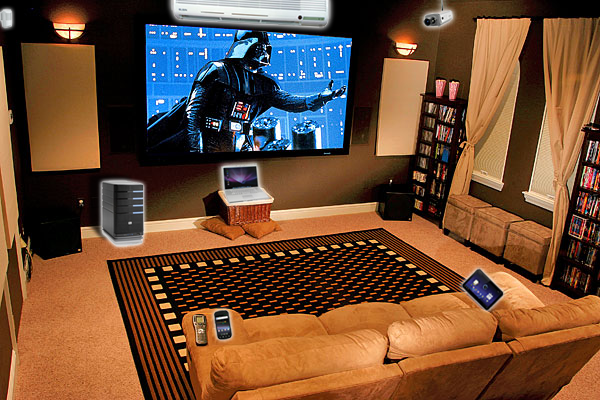
\includegraphics[scale=0.7]{imagens/salaUbiqua}
	\caption{Exemplo de ambiente inteligente.}
	\label{fig:ambienteInteligente}
\end{figure}

Em um ambiente inteligente se faz necessária a adaptabilidade de serviços de forma transparente para os clientes, ou seja, caso um serviço não esteja mais sendo provido por determinado dispositivo, o \emph{smart space} deve identificar esta falha e procurar um outro servidor ~\cite{gomes2007, passarinho2008, paranhos2009}.

\section{DSOA}

Com o objetivo de auxiliar a modelagem de um \emph{smart space} levando em consideração as características de um ambiente ubíquo, foi criada a arquitetura DSOA(\emph{Device Service Oriented Architecture})~\cite{buzetoDSOA2010} que faz uso dos conceitos definidos na SOA(\emph{Service Oriented Architecture}) aplicados a um ambiente inteligente, onde recursos e serviços estarão disponíveis de forma dinâmica. Recursos, segundo a definição na proposta da DSOA, são um grupo de funcionalidades logicamente relacionadas que deverão ser acessíveis por meio de interfaces pré-definidas ~\cite{buzeto2010}. 

Esses recursos serão acessados por meio do \emph{middleware} \emph{uOS}, que utiliza um conjunto de protocolos \emph{uP} (\emph{Ubiquitous Protocols}) como interface de comunicação com \emph{drivers} de recursos disponíveis. A infra-estrutura implementada pelo \emph{uOS} para gerir os recursos do ambiente permite que uma aplicação de um dispositivo acesse recursos, apresentados na forma de um \emph{driver} (\emph{UosDriver}) de outros dispositivos presentes no ambiente.

Quando uma aplicação solicita um serviço de algum recurso, o \emph{uOS} deve tomar uma decisão sobre qual será o dispositivo detentor de tal recurso que provê o serviço solicitado que irá ser escolhido. Para que o \emph{uOS} possa tomar uma decisão inteligente sobre a escolha do dispositivo detentor do recurso, deseja-se que o tipo do recurso seja conhecido. Atualmente, a arquitetura DSOA/\emph{uOS} é pouco maleável nessa definição de tipo de recursos. Os recursos são definidos de forma linear, por exemplo: um recurso de \emph{mouse} com dois botões possui um \emph{driver} associado, já um \emph{mouse} com três botões, possui um outro \emph{driver} associado que não possui nenhuma relação com o primeiro, o que dificulta a tomada de decisão por parte do \emph{middleware}. Existem diversos padrões definidos que fazem uso de uma classificação de dispositivos ou recursos, mas não se adequam à arquitetura DSOA.

O objetivo deste trabalho é definir uma classificação de recursos e a partir desta classificação, prover uma hierarquia de recursos extensível para a arquitetura DSOA do \emph{middleware} de Computação Ubíqua \emph{uOS}. Essa hierarquia irá facilitar a escolha de determinado serviço provido por algum recurso por parte do \emph{uOS} ou de alguma aplicação cliente.

O presente trabalho encontra-se organizado da seguinte maneira: o capítulo 2 fundamenta os conceitos que serão utilizados neste trabalho e apresenta uma visão geral do projeto UbiquitOS, a arquitetura DSOA e o conjunto de protocolos \emph{uP}. O capítulo seguinte descreve a importância da classificação de recursos, bem como as diferentes maneiras de se representa-la. Lista também os principais padrões conhecidos e projetos que utilizam uma classificação para auxilio de suas atividades.
\end{comment}

O restante deste trabalho está organizado da seguinte maneira: O Capítulo 2 fundamenta os conceitos que serão utilizados no decorrer deste documento. O Capítulo 3 apresenta a classificação de recursos proposta por este trabalho. O Capítulo 4 detalha a implementação da classificação de recursos no \emph{middleware} \emph{uOS} e mostra o estudo de caso realizado para demonstrar uma adequada utilização da classificação de recursos. Por fim, o Capítulo 5 apresenta a conclusão e trabalhos futuros.

\begin{comment}
Cap. 2
Apresenta-se inicialmente uma visão geral do projeto UbiquitOS, explicando os principais conceitos da DSOA e mostrando em detalhes os protocolos que constituem o uP. A seção seguinte mostra a importância da classificação de recursos bem como as diferentes maneiras de se classificar e representá-la. Ainda na segunda seção, serão apresentados alguns dos principais padrões conhecidos e projetos de Computação Ubíqua que utilizam uma classificação de recursos ou dispositivos para auxiliar em suas atividades. A seção e o capítulo são finalizados realizando um comparativo entre as diferentes classificações mostradas. 

Cap. 3
Na primeira seção serão mostrados os tipos básicos definidos pela classificação, o identificador e seus serviços associados. A seção seguinte apresenta o conceito da similaridade de recursos e como é estabelecida uma relação de similaridade entre recursos. O capítulo é concluído detalhando os impactos dessa classificação na arquitetura DSOA/\emph{uOS}.
\end{comment}